%%%%%%%%%%%%%%%%%%%%%%%%%%%%%%%%%%%%%%%%%%%%%%%%%%%%%%%%
% 							                   PREAMBULE        
%%%%%%%%%%%%%%%%%%%%%%%%%%%%%%%%%%%%%%%%%%%%%%%%%%%%%%%%

\documentclass[a4,12pt]{article}

%--- Packages génériques ---%

\usepackage[francais]{babel}
\usepackage[utf8]{inputenc}
\usepackage[T1]{fontenc}
\usepackage[babel=true]{csquotes}
\usepackage{amsmath}
\usepackage{amssymb}
\usepackage{float}
\usepackage{graphicx}
\usepackage{hyperref}

%--- Structure de la page ---%

\usepackage{fancyheadings}

\topmargin -1.5 cm
\oddsidemargin -0.5 cm
\evensidemargin -0.5 cm
\textwidth 17 cm
\setlength{\headwidth}{\textwidth}
\textheight 24 cm
\pagestyle{fancy}
\lhead[\fancyplain{}{\thepage}]{\fancyplain{}{\sl ENSIMAG 2A}}
\chead[\fancyplain{}{{\sl }}]{\fancyplain{}{{TP Traitement d'Image}}}
\rhead[\fancyplain{}{}]{\fancyplain{}{Loiodice \& Vincent}}
\lfoot{\fancyplain{}{}}
\cfoot{\fancyplain{}{}}
\cfoot{\thepage }
\rfoot{\fancyplain{}{}}

%--- Style de la zone de code ---%

\usepackage{tikz}
\usetikzlibrary{calc}
\usepackage[framemethod=tikz]{mdframed}
\usepackage{listings}             
\usepackage{textcomp}

\lstset{upquote=true,
        columns=flexible,
        keepspaces=true,
        breaklines,
        breakindent=0pt,
        basicstyle=\ttfamily,
        commentstyle=\color[rgb]{0,0.6,0},
        language=Scilab,
        alsoletter=\),
        }

\lstset{classoffset=0,
        keywordstyle=\color{violet!75},
        deletekeywords={zeros,disp},
        classoffset=1,
        keywordstyle=\color{cyan},
        morekeywords={zeros,disp},
        }

\lstset{extendedchars=true,
        literate={0}{{\color{brown!75}0}}1 
                 {1}{{\color{brown!75}1}}1 
                 {2}{{\color{brown!75}2}}1 
                 {3}{{\color{brown!75}3}}1 
                 {4}{{\color{brown!75}4}}1 
                 {5}{{\color{brown!75}5}}1 
                 {6}{{\color{brown!75}6}}1 
                 {7}{{\color{brown!75}7}}1 
                 {8}{{\color{brown!75}8}}1 
                 {9}{{\color{brown!75}9}}1 
                 {(}{{\color{blue!50}(}}1 
                 {)}{{\color{blue!50})}}1 
                 {[}{{\color{blue!50}[}}1 
                 {]}{{\color{blue!50}]}}1
                 {-}{{\color{gray}-}}1
                 {+}{{\color{gray}+}}1
                 {=}{{\color{gray}=}}1
                 {:}{{\color{orange!50!yellow}:}}1
                 {é}{{\'e}}1 
                 {è}{{\`e}}1 
                 {à}{{\`a}}1 
                 {ç}{{\c{c}}}1 
                 {œ}{{\oe}}1 
                 {ù}{{\`u}}1
                 {É}{{\'E}}1 
                 {È}{{\`E}}1 
                 {À}{{\`A}}1 
                 {Ç}{{\c{C}}}1 
                 {Œ}{{\OE}}1 
                 {Ê}{{\^E}}1
                 {ê}{{\^e}}1 
                 {î}{{\^i}}1 
                 {ô}{{\^o}}1 
                 {û}{{\^u}}1 
        }

%--- Raccourcis commande ---%

\newcommand{\R}{\mathbb{R}}
\newcommand{\N}{\mathbb{N}}
\newcommand{\A}{\mathbf{A}}
\newcommand{\B}{\mathbf{B}}
\newcommand{\C}{\mathbf{C}}
\newcommand{\D}{\mathbf{D}}
\newcommand{\ub}{\mathbf{u}}

%--- Mode correction et incréments automatiques ---%

\usepackage{framed}
\usepackage{ifthen}
\usepackage{comment}
\usepackage{graphicx}

\newcounter{Nbquestion}

\newcommand*\question{%
\stepcounter{Nbquestion}%
\textbf{Question \theNbquestion. }}

\newboolean{enseignant}
%\setboolean{enseignant}{true}
\setboolean{enseignant}{false}

\definecolor{shadecolor}{gray}{0.80}

\ifthenelse{
\boolean{enseignant}}{
\newenvironment{correction}{\begin{shaded}}{\end{shaded}}
}
{
\excludecomment{correction}
}

%--- Style de l'encadré des questions ---%

\mdfsetup{leftmargin=12pt}
\mdfsetup{skipabove=\topskip,skipbelow=\topskip}

\tikzset{
	warningsymbol/.style={
	rectangle,draw=red,
	fill=white,scale=1,
	overlay}}
\global\mdfdefinestyle{exampledefault}{
	hidealllines=true,leftline=true,
	innerrightmargin=0.0em,
	innerleftmargin=0.3em,
	leftmargin=0.0em,
	linecolor=red,
	backgroundcolor=orange!20,
	middlelinewidth=4pt,
	innertopmargin=\topskip,
}

\global\mdfdefinestyle{answer}{
	hidealllines=true,leftline=true,
	innerrightmargin=0.0em,
	innerleftmargin=0.3em,
	leftmargin=0.0em,
	linecolor=green,
	backgroundcolor=white,
	middlelinewidth=4pt,
	innertopmargin=\topskip,
}

%%%%%%%%%%%%%%%%%%%%%%%%%%%%%%%%%%%%%%%%%%%%%%%%%%%%%%%%
% 							               EN-TETE        
%%%%%%%%%%%%%%%%%%%%%%%%%%%%%%%%%%%%%%%%%%%%%%%%%%%%%%%%

\title{\textbf{TP2 Traitement d'Image\\Filtrage non linéaire}}
\author{
\begin{tabular}{cc}
	\textsc{Loiodice Thomas} & \textsc{Vincent Kylian} \\
\end{tabular}}   
\date{\small \today}

\makeatletter
	\def\thetitle{\@title}
	\def\theauthor{\@author}
	\def\thedate{\@date}
\makeatother 

\usepackage{etoolbox}
\usepackage{titling}
\setlength{\droptitle}{-7em}

\setlength{\parindent}{1cm}

\makeatletter
% patch pour le bug concernant les parenthèses fermantes d'après http://tex.stackexchange.com/q/69472
\patchcmd{\lsthk@SelectCharTable}{%
  \lst@ifbreaklines\lst@Def{`)}{\lst@breakProcessOther)}\fi}{}{}{}
  
%%%%%%%%%%%%%%%%%%%%%%%%%%%%%%%%%%%%%%%%%%%%%%%%%%%%%%%%
% 							CORPS DU DOCUMENT          
%%%%%%%%%%%%%%%%%%%%%%%%%%%%%%%%%%%%%%%%%%%%%%%%%%%%%%%%

\begin{document}
\maketitle


%%%%%%%%%%%%%%%%%%%%%%%%%%%%%%%%%%%%%%%%%%%%%%%%%%%%%%%%
% 						                  	PARTIE I         
%%%%%%%%%%%%%%%%%%%%%%%%%%%%%%%%%%%%%%%%%%%%%%%%%%%%%%%%

\section{Partie I : Implémentation et estimation des paramètres}

Tout d'abord, nous avons décidé de travailler sur des images prolongées par miroir, afin de pouvoir avoir en sortie une image de même taille qu'en entrée. Cela permet d'avoir un filtre pleinement fonctionnel. Pour cela nous avons créé une fonction dédiée permettant de ramener les indices en dehors de la taille de l'image aux valeurs identiques en miroir.

\subsection{Filtre Médian}

Le filtre médian donne généralement un bon résultat pour un $n$
compris entre 2 et 5. Il a l'avantage d'être rapide $ \approx 0.1 s $
pour un filtre de taille raisonnable et son temps s'accroît linéairement 
avec la taille de l'image.
En s'appuyant sur la métrique du PSNR, la meilleure demi-taille du filtre est généralement 3,
ce que confirme notre observation qualitative. 
Le défaut principal de ce filtre est qu'il a tendance a lisser les surfaces. 
En effet plus la taille du filtre est importante plus le résultat est déformé.
Il est donc inutile de prendre un filtre médian de taille trop grande.

\subsection{Filtre Adaptatif Récursif}
Dans le cas de ce filtre, le critère d'arrêt est un élément très important. En effet ce dernier doit être bien défini et estimé pour permettre un filtrage complet sans effectuer d'étapes superflues. Pour cela, l'arrêt est défini sur l'écart (norme 2 sur la différence) entre deux traitements successifs d'images. L'écart seuil a été fixé empiriquement après essais sur les différentes images de test. Nous avons cependant remarqué que le choix du paramètre k de filtrage influe très fortement sur ce critère d'arrêt. En effet, si ce dernier est mal dimensionné face au niveau de bruit de l'image alors un point fixe est très difficile à atteindre. Dans ce cas l'exécution est stoppée à 200 itérations, valeur jugée suffisante au regard des essais effectués et de la description du filtre.\\

Dans le cas d'une valeur de $k$ trop importante, les contours se retrouvent découpés trop grossièrement : les bords des formes sont ainsi arrondis et les surfaces des formes internes se voient diminuer.\\

Il n'est pas possible, pour ce filtre, de donner une valeur de K générique fonctionnant de manière optimale pour les différents types et intensités de bruit, K dépendant en effet de ce niveau de bruit. Les valeurs préconisées pour ce paramètre sont comprises entre  10 (faibles bruits) et 50 (forts bruits). Pour trouver ces valeurs nous avons étudié la convergence des images vers un point fixe en affichant la différence entre deux images successives.
\subsection{Filtre Bilatéral}

Le filtrage par filtre bilatéral dépend de deux paramètres $\sigma_1$ et $\sigma_2$. 
Le concept est d'appliquer à l'image une gaussienne en distance et en intensité puis de normaliser le filtrage.
La gaussienne en distance réalise un lissage (niveau de détails). 
Celle en intensité permet de ne lisser que par zones de couleurs similaires et donc de conserver les contours.
Ainsi, prendre $\sigma_2$ grand donne beaucoup d'importance aux contours, 
on conserve un grand niveau de détail, 
l'inverse conduit cependant à flouter l'image.\\

Le temps de calcul du filtre ne dépend pas de $\sigma_2$,
il est donc possible (et important) de choisir une valeur adaptée au niveau de détail que l'on souhaite conserver.
$\sigma_1$ , lui, détermine la taille du filtre. 
Son accroissement a une répercussion quadratique sur le temps de calcul.
Il sera alors préférable qu'il ne soit pas trop grand. 
Pour $\sigma_1 = 3 $ on obtient un résultat acceptable pour un temps d'exécution ne dépassant 10 seconde.
Pour $\sigma_1 = 5 $ on atteint déjà la minute de calcul pour une légère amélioration.\\


\noindent
\begin{minipage}[c]{0.33\linewidth}
	\begin{center}
		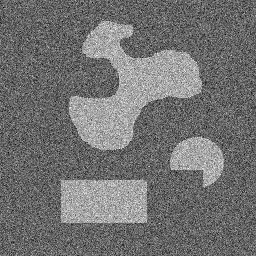
\includegraphics[width = 40mm]{./img/formOrig.jpg}\\
		\textit{Image originale}\\
	\end{center}
\end{minipage}
\begin{minipage}[c]{0.33\linewidth}
	\begin{center}
		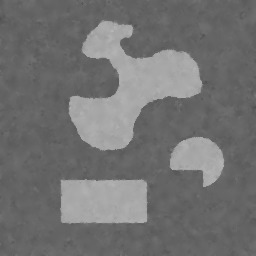
\includegraphics[width = 40mm]{./img/formbb25Bil3_20.jpg}\\
		\textit{$\sigma_1=3, \sigma_2=20$}\\
	\end{center}
\end{minipage}
\begin{minipage}[c]{0.33\linewidth}
	\begin{center}
		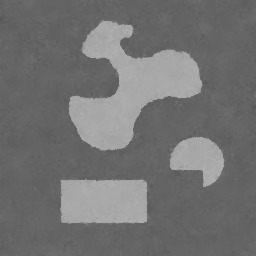
\includegraphics[width = 40mm]{./img/formbb25Bil5_20.jpg}\\
		\textit{$\sigma_1=5, \sigma_2=20$}\\
	\end{center}
\end{minipage}\\

\hspace{2em}

Concernant le PSNR, il s'accroît de plus en plus faiblement avec $\sigma_1$ (nous avons testé jusqu'à $\sigma_1 = 17$ , pour un $\sigma_2 \approx 10$ )
Le PSNR tend alors vers 40.\\
Pour la suite on considérera  $\sigma_1 = 5$ ,pour un $\sigma_2 \approx 10$ comme valeur acceptable pour un filtre bilateral, permettant ainsi un bon compromis entre temps de calcul et résultats obtenus.

\subsection{Filtre NL-Means}
Concernant le filtrage NL-Means, l'estimation du meilleur choix de taille de patchs et de région est difficile. En effet le filtre est très coûteux en calculs et rend les tests de différentes valeurs très longs, augmentant avec la taille de ces derniers. Nous avons effectué quelques essais qui nous ont permis d'aboutir à un compromis qui nous a semblé satisfaisant en prenant un taille de patchs \textit{r = 5} et une taille de région \textit{t = 10}. En effet, sur l'exemple de l'image \textit{formes2bb10.pgm} l'écart (de PSNR et visuel) est très faible avec une taille de patchs \textit{r = 5} et une taille de région \textit{t = 15} (\textit{PSNR = 40.01} contre $40.02$ avec les tailles précédentes). Cependant le temps de calcul est, lui, fortement augmenté : respectivement \textit{3m44.028s} (pour \textit{r=5, t=10}) et \textit{1m39.620s} (\textit{r=7, t=15}).\\

Ces valeurs sont ainsi intéressantes pour la plupart des valeurs de bruit gaussien, mais il est quelquefois nécessaire de les augmenter (au prix d'un plus grand nombre de calculs) si le niveau de bruit est trop fort. Cela permet d' améliorer la robustesse de la méthode : les patchs comparés sont alors plus grands, réduisant l'incidence du bruit sur les formes recherchées.\\

Pour les autres types de bruit (speckle et poivre et sel), des tailles inférieures pour le patch et la région nous ont semblé donner de meilleurs résultats. En effet, ces bruits présentent une forte variance décorrélée de l'image et rendent la recherche sur un grand voisinage trop aléatoire du fait de la forte différence possible entre deux pixels successifs.\\

Cependant ces tailles ne doivent pas être trop faibles, sans quoi des variations restent perceptibles dans les zones homogènes, il est alors nécessaire de rehausser la valeur du lissage $\sigma$ pour compenser cet effet :\\

\noindent
\begin{minipage}[c]{0.50\linewidth}
	\begin{center}
		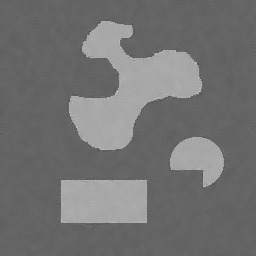
\includegraphics[width = 50mm]{./img/nltroppetit4-2-10.jpg}\\
		\textit{$t=4, r=2, \sigma=10$}\\
	\end{center}
\end{minipage}
\begin{minipage}[c]{0.50\linewidth}
	\begin{center}
		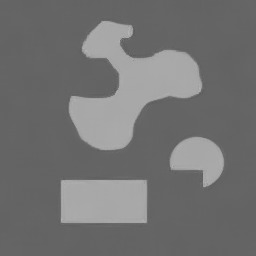
\includegraphics[width = 50mm]{./img/nlassezgrand10-5-10.jpg}\\
		\textit{$t=10, r=5, \sigma=10$}\\
	\end{center}
\end{minipage}\\
\\
\subsection{Estimation du bruit}
Dans le cas de l'implémentation du bruit, et pour se rapprocher des valeurs données en exemple dans le sujet (seuil de 60) nous avons jugé plus pertinent de renvoyer la valeur de l'écart type plutôt que la variance en elle-même ($\sigma = \sqrt{V}$).


\section{Partie II : Comparaison des filtres}
\subsection{Comparaison quantitative}

Les tests suivants ont été effectués sur plusieurs images, présentant un bruit ou une intensité de bruit différente. Les images des différents bruits ont été choisis de manière à avoir une variance uniforme entre les différents types (variance calculée identique pour les trois derniers bruits), permettant ainsi une bonne comparaison.\\

Dans chaque cas le test a été effectué dans le but d'obtenir un PSNR maximal (choix des paramètres en conséquence). C'est pour ce PSNR obtenu que le temps CPU est mesuré. Les temps ainsi mesurés ont été moyennés sur 5 réalisations. Les valeurs renseignées pour le filre NL-Means sont dans l'ordre : $t$ (région), $r$ (patchs), $\sigma$.\\

Image \textit{formes2bb10.pgm}, présentant un faible bruit gaussien (Estimation de bruit : 22.27).

\begin{center}
\begin{tabular}{|l||c|c|c|c|}
\hline
formes2bb10 & Filtre Médian & Filtre Adaptatif & Filtre Bilatéral & Filtre NL-Means \\
& n=3 & k=12 & $\sigma_1 = 5$ $\sigma_2 = 17$ & 10,5,10\\
\hline
Estimation du bruit
& 4.99
& 2.38
& 2.60
& 2.60\\
\hline
PSNR
& 36.12
& 40.85
& 44.18
& 40.02\\
\hline
Temps CPU
& 0.04s 
& 1.002s
& 31.73s
& 1m20.23s\\
\hline
\end{tabular} 
\end{center}

\vspace{2em}

Image \textit{formes2bb67.pgm}, présentant un fort bruit gaussien (Estimation de bruit : 180.25).

\begin{center}
\begin{tabular}{|l||c|c|c|c|}
\hline
formes2bb67 & Filtre Médian & Filtre Adaptatif & Filtre Bilatéral & Filtre NL-Means\\
& n=8 & k=36 & $\sigma_1 = 5$ $\sigma_2 = 108$ & 11,6,49\\
\hline
Estimation du bruit
& 10.63
& 5.82
& 9.45
& 8.64\\
\hline
PSNR
& 27.07
& 25.02
& 27.66
& 27.17\\
\hline
Temps CPU
& 0.05s
& 3.345s
& 50.7s
& 1m19.92s\\
\hline
\end{tabular} 
\end{center}

\vspace{2em}

Image \textit{formes2pets5.pgm}, présentant un fort bruit poivre et sel (Estimation de bruit : 150.13).

\begin{center}
\begin{tabular}{|l||c|c|c|c|}
\hline
formes2pets5  & Filtre Médian & Filtre Adaptatif & Filtre Bilatéral & Filtre NL-Means\\
& n=2 & k=32 & $\sigma_1 = 5$ $\sigma_2 = 15$ & 6,4,39\\
\hline
Estimation du bruit
& 1.56
& 4.38
& 8.10
& 16.87\\
\hline
PSNR
& 34.17
& 25.23
& 27.95
& 26.15\\
\hline
Temps CPU
& 0.03s
& 3.321s
& 20.14s
& 22.897s\\
\hline
\end{tabular} 
\end{center}

\vspace{2em}

Image \textit{formes2sp5.pgm}, présentant un fort bruit speckle (Estimation de bruit : 170.18).

\begin{center}
\begin{tabular}{|l||c|c|c|c|}
\hline
formes2sp5  & Filtre Médian & Filtre Adaptatif & Filtre Bilatéral & Filtre NL-Means \\
& n=9 & k=48 & $\sigma_1 = 5$ $\sigma_2 = 170$ &6,5,91\\
\hline
Estimation du bruit
& 10.58
& 4.38
& 8.17
& 11.64\\
\hline
PSNR
& 25.27
& 23.80
& 26.01
& 25.86\\
\hline
Temps CPU
& 0.05s
& 3.346s
& 49.6s
& 28.691s\\
\hline
\end{tabular} 
\end{center}

On remarque tout que le filtre NL-Means, bien qu'offrant des résultats très satisfaisants est bien plus long que les autres filtres. Il est possible de diminuer son temps d'exécution en prenant des régions plus petites (par ex. $t=4$, $r=2$) au prix d'une augmentation du facteur de lissage $\sigma$ et d'un moins bon filtrage (l'ordre de temps est alors inférieur à 10s et se rapproche de ceux obtenus pour les autres filtres).\\

Le filtre Bilatéral semble être intéressant, présentant un coût modéré pour un résultat surpassant les autres filtres en se basant sur le PSNR. C'est cependant le filtre adaptatif récursif qui semble donner les meilleurs résultats au regard de l'estimation du bruit.\\

Ainsi il semblerait que parmi ces deux filtres, le filtre adaptatif récursif parvienne à un meilleur lissage du bruit que le bilatéral mais en étant moins fidèle à l'image d'origine que ce dernier. Les estimateurs numériques ne donnant que peu d'appréciation sur ces hypothèses nous les vérifierons lors de l'étude qualitative.\\

Enfin, le filtre médian, bien qu'étant le plus rapide, est très irrégulier. En effet sur certaines images ou sur le bruit "poivre et sel" il semble donner de meilleurs résultats que les autres filtres mais cela ne se vérifie pas pour d'autre types d'images comme on peut le voir avec l'image de faible bruit gaussien \textit{formes2bb10.pgm}.


\vspace{2em}

\subsection{Comparaison qualitative}

Nous avions vu lors du TP précédent que le PSNR permet d'avoir une idée générale mais qu'une estimation visuelle permet de trouver un meilleur compromis entre le bruit persistant et la conservation des contours de l'image. La comparaison visuelle qualitative apparaît donc indispensable.\\

Nous avons choisi l'image \textit{globulesbb25.pgm} afin d'avoir une image présentant plus de critères de comparaison que les formes précédentes (dégradés de couleur, contours, niveaux de couleur...). Cette image présente un bruit gaussien moyen, d'une variance estimée à $54.25$. Les résultats obtenus pour les différents filtres sont les suivants :\\


\noindent
\begin{center}
	\begin{minipage}[c]{0.45\linewidth}
		\begin{center}
			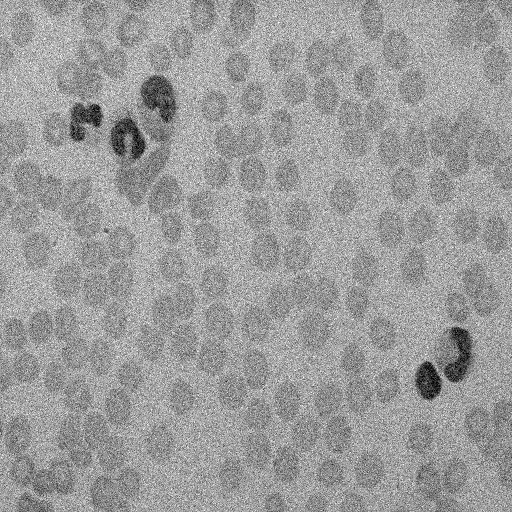
\includegraphics[width = 70mm]{./img/globOrig.jpg}
			\textit{Image d'origine}
		\end{center}
	\end{minipage}
\end{center}

\noindent
\begin{center}
	\begin{minipage}[c]{0.45\linewidth}
		\begin{center}
			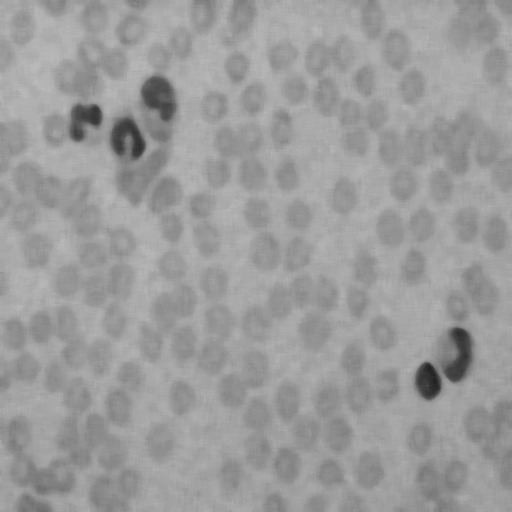
\includegraphics[width = 70mm]{./img/globb25Med4.jpg}
			\textit{Filtre Médian}\\
			\textit{$n=4$}\\
                        \hspace{2em}
		\end{center}
	\end{minipage}
	\begin{minipage}[c]{0.45\linewidth}
		\begin{center}
			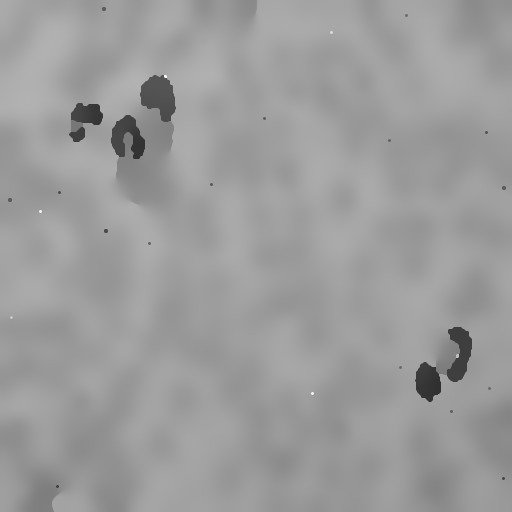
\includegraphics[width = 70mm]{./img/globAdapt12.jpg}
			\textit{Filtre Adaptatif}\\
			\textit{$K = 12$}\\
                        \hspace{2em}
		\end{center}
	\end{minipage}
	\begin{minipage}[c]{0.45\linewidth}
		\begin{center}
			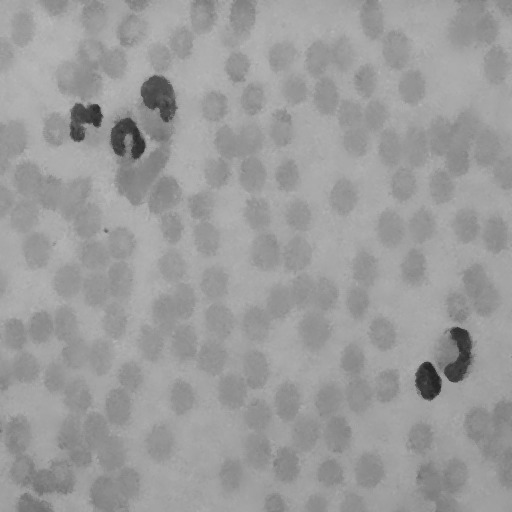
\includegraphics[width = 70mm]{./img/globb25Bilateral_5_20.jpg}
			\textit{Filtre Bilatéral}\\
			\textit{$\sigma_1 =5 , \sigma_2=20$}\\
		\end{center}
	\end{minipage}
	\begin{minipage}[c]{0.45\linewidth}
		\begin{center}
			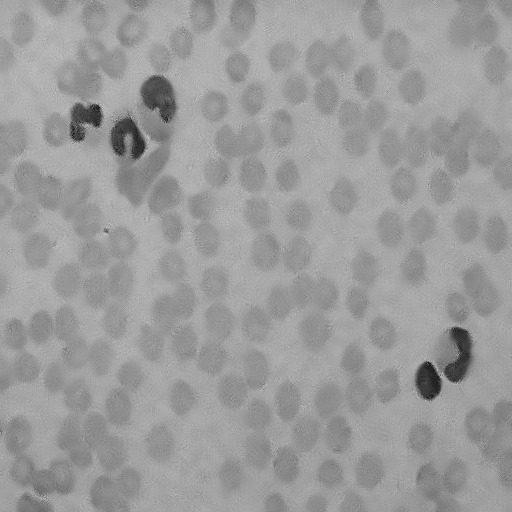
\includegraphics[width = 70mm]{./img/globNLMeans.jpg}
			\textit{Filtre NL-Means}\\
			\textit{$t = 6, r= 3, \sigma=15$}\\
		\end{center}
	\end{minipage}\\
\end{center}


On remarque tout d'abord que le filtre adaptatif récursif ne donne pas d'aussi bons résultats que les autres filtres, contrairement à ce qu'on a vu avec l'étude numérique précédente. En effet on n'obtient qu'un résultat fortement flouté avec seulement le détachement des formes les plus sombres.

La condition d'arrêt du nombre d'itérations semble être en cause, en effet en bridant l'algorithme à 7 itérations on obtient un résultat bien plus satisfaisant :\\

\noindent
\begin{center}
	\begin{minipage}[c]{0.45\linewidth}
		\begin{center}
			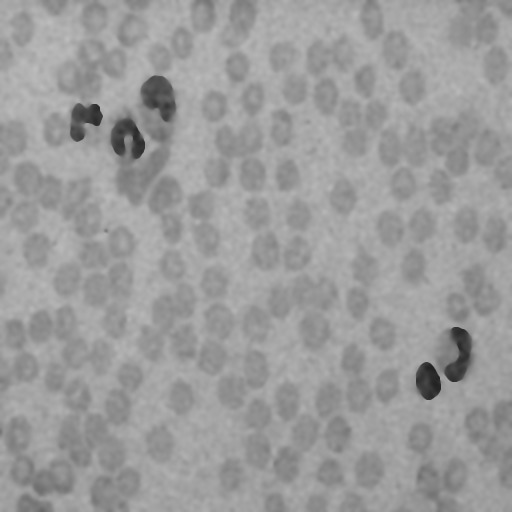
\includegraphics[width = 70mm]{./img/globAdaptMoinsInt.jpg}
			\textit{Filtre Adaptatif}
			\textit{$K = 35, 7$ itérations}\
		\end{center}
	\end{minipage}
\end{center}

Nous n'avons cependant pas réussi à affiner le calcul d'un critère d'arrêt qui permette de bons résultats que ce soit sur les images de globules et les images \textit{formesAxxyy} qui, elles, nécessitent comme expliqué dans le sujet un plus grand nombre d'itérations (100 à 200 généralement).\\


Concernant les autres filtres, le filtre NL-Means semble donner les meilleurs résultats. Les autres filtres donnent cependant un résultat assez proche et pour un coût de calcul bien inférieur. C'est notamment le cas pour les filtres "Adaptatif Récursif" et "Bilinéaire" qui permettent un très bon compromis entre une suppression du bruit et une conservation des contours. L'hypothèse vue en section précédente pour ces deux filtres semble se vérifier sur ces images (adaptatif offrant un résultat plus lisse mais possiblement moins fidèle aux colorations d'origine).\\


Le filtre médian semble rester en retrait à cause de la déformation des contours qu'il entraîne.

% Fin section 2 %
\end{document}

% Fin du document LaTeX
